\section{Robot Design (Sergio)}

During the design and assembly stage, two models where proposed. The first prototype used caterpillar wheels, robust body and a sensor on the top with 360$^{\circ}$ of freedom. The second and current model,conversely, is lighter with the sensor suited at the bottom with 180$^{\circ}$ of freedom. It presents the following advantages: 

1) Lightweight. The main robot pieces are the motors, these parts are used as frame to support the body and the NXT control.


2) Compact. The first prototype had a long body because the NXT control was in a horizontal position. This design presented two main problems, difficulties to turn and a considerable error range while rotating. In order to remove these issues the NXT control was placed in vertical position secured by few pieces to the motors.

3) Fast. Taking into account the previous points the robot's movements resulted to be quick and accurate. An improvement was made using a tail to provide more stability and reducing the friction while rotating. 

Images of the final version can be seen in Figure 1.


\begin{figure}[h!]
	\centering
	\begin{subfigure}[b]{0.3\textwidth}
		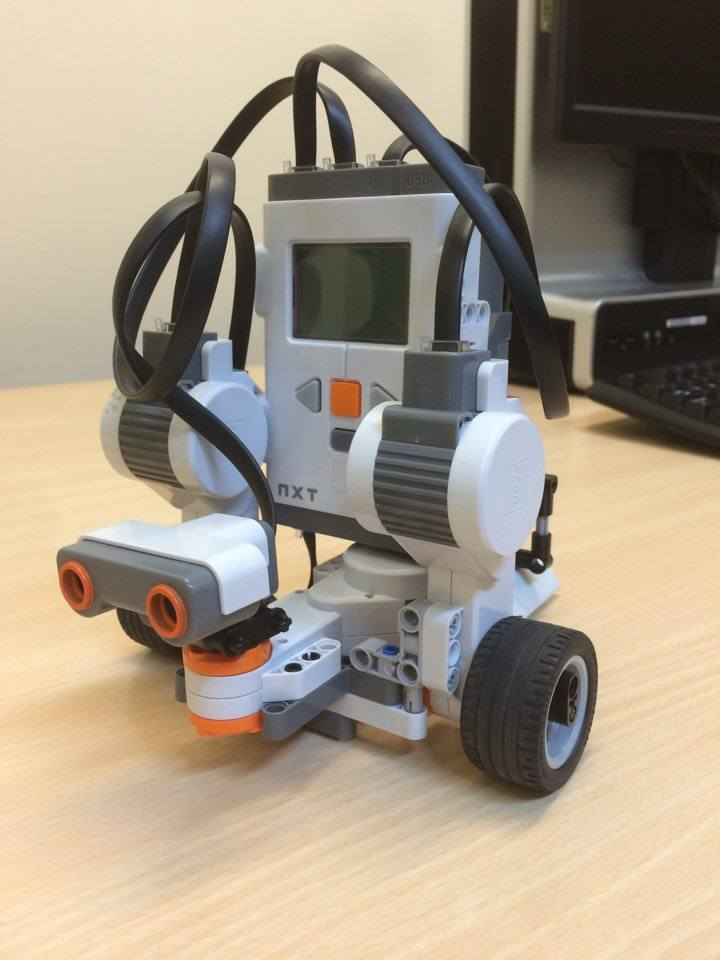
\includegraphics[width=\textwidth]{robot1}
		\caption{Front}
		\label{fig:front}
	\end{subfigure}
	~ %add desired spacing between images, e. g. ~, \quad, \qquad, \hfill etc. 
	%(or a blank line to force the subfigure onto a new line)
	\begin{subfigure}[b]{0.3\textwidth}
		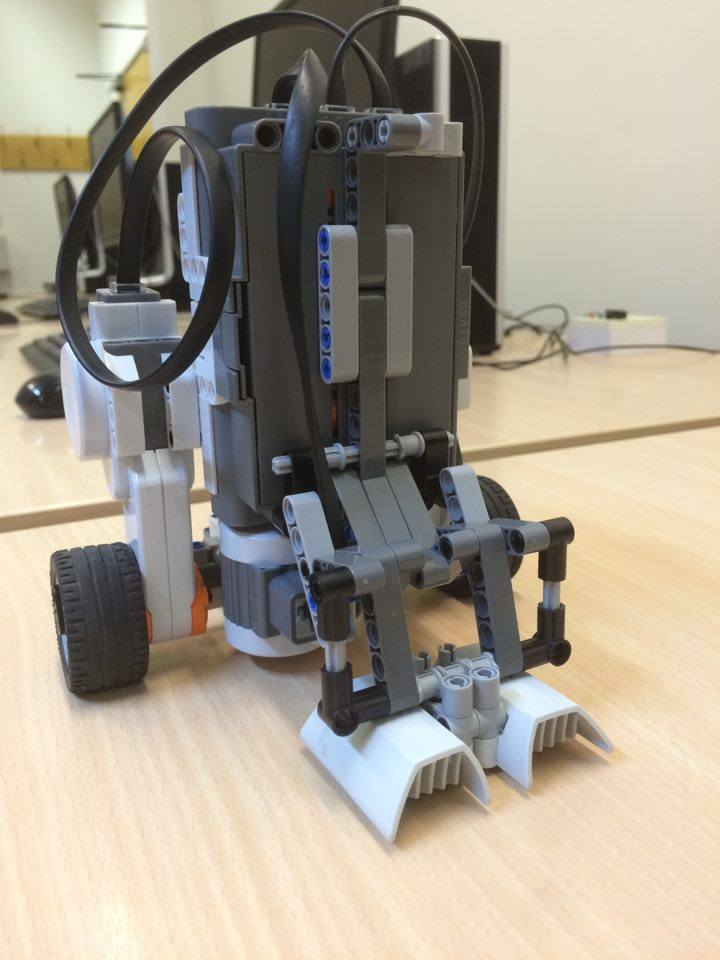
\includegraphics[width=\textwidth]{robot2}
		\caption{Back}
		\label{fig:back}
	\end{subfigure}
	~ 
	\begin{subfigure}[b]{0.3\textwidth}
		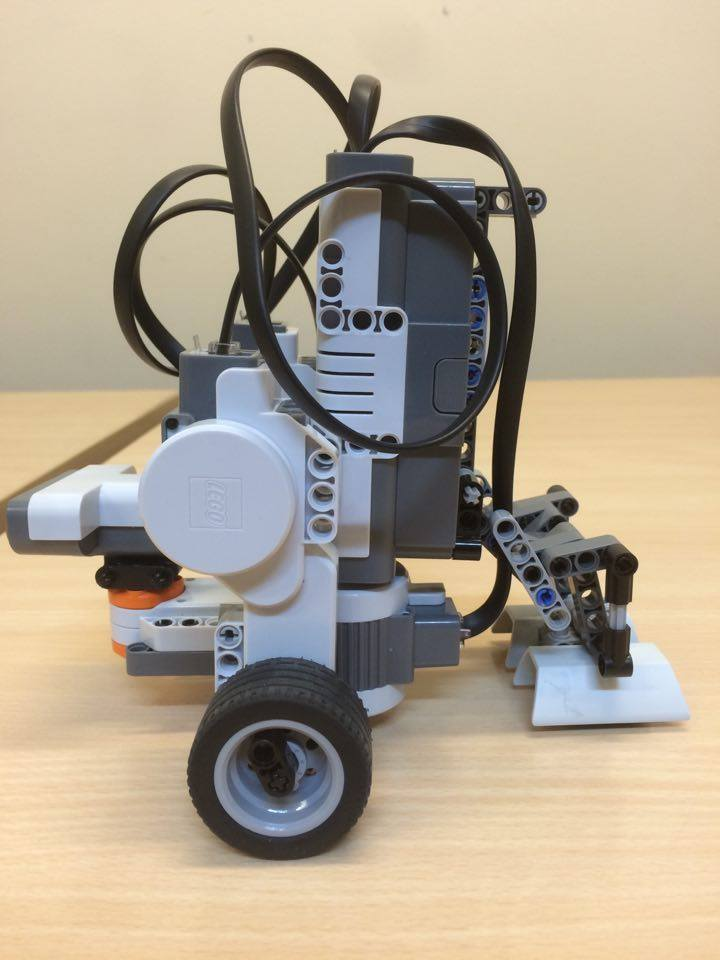
\includegraphics[width=\textwidth]{robot3}
		\caption{Side}
		\label{fig:side}
	\end{subfigure}
	\caption{Robot design views}\label{fig:robot}
\end{figure}


\FloatBarrier


\section{Robot configuration (Kevin)}
% describe the design
% what are the advantages
We mainly focus on two aspects when configuring the Lego robot, namely {\itshape \rom{1})} stability and {\itshape \rom{2})} feasibility. The complete configuration of the robot is visualised in Fig.\ref{fig:robotconfig}, where there are three images showing the front, side and back appearances of the robot respectively. 

The total height of the robot is approximately 18 cm. The width and length are 13 cm and 19.5 cm, respectively. This configuration ensures that the robot does not occupy too much space in the arena. The ultrasonic sensor, which is the only sensor being used, is placed in the lower front with an approximate height of 6.5 cm and has a vision range of 180 degrees. Using a 360 degree of freedom seems to be more useful but we do not employ this design since the wire connecting the sensor with the brick influences the turning of the sensor. A novel feature used in this design is the support device installed in the back as shown in Fig.\ref{fig:backrobot}, where two balls are positioned inside the two white slots to reduce the friction between the ground and the support device. 

\begin{figure}[h]
\centering
  \begin{subfigure}{0.25\textwidth}
  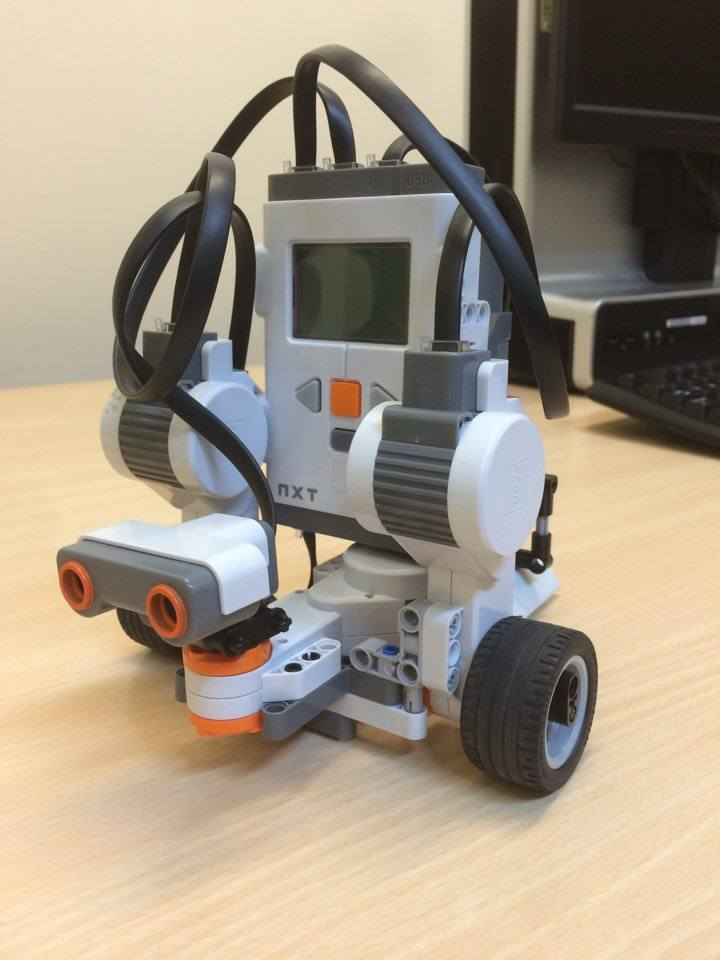
\includegraphics[scale=0.15]{f}
  \caption{Front appearance}
  \end{subfigure}
  \begin{subfigure}{0.25\textwidth}
  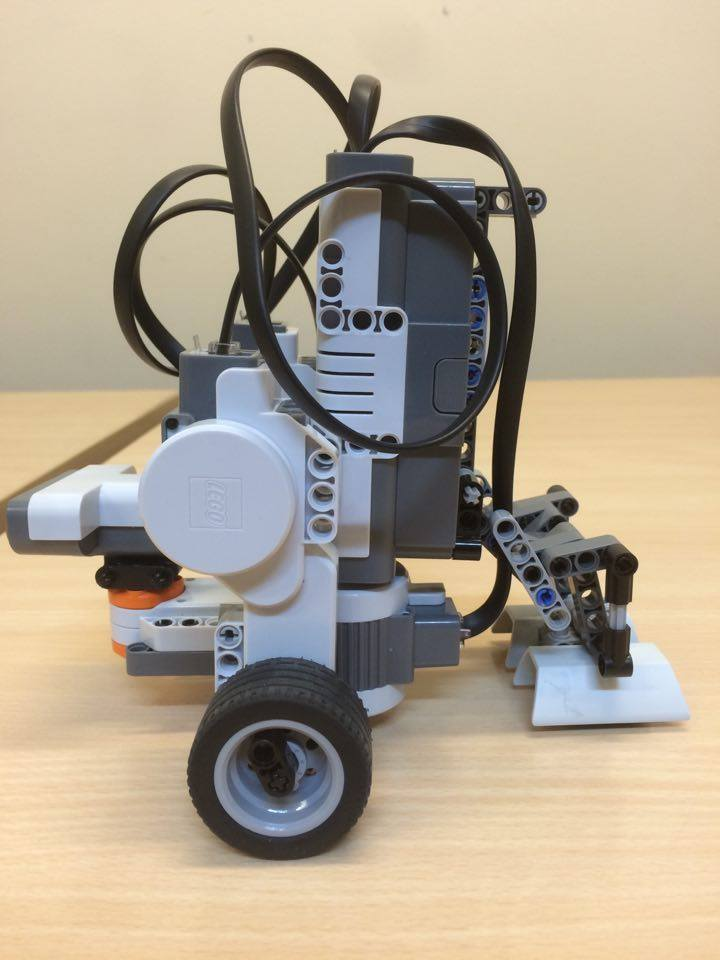
\includegraphics[scale=0.15]{s}
  \caption{Side appearance}
  \end{subfigure}
  \begin{subfigure}{0.25\textwidth}
  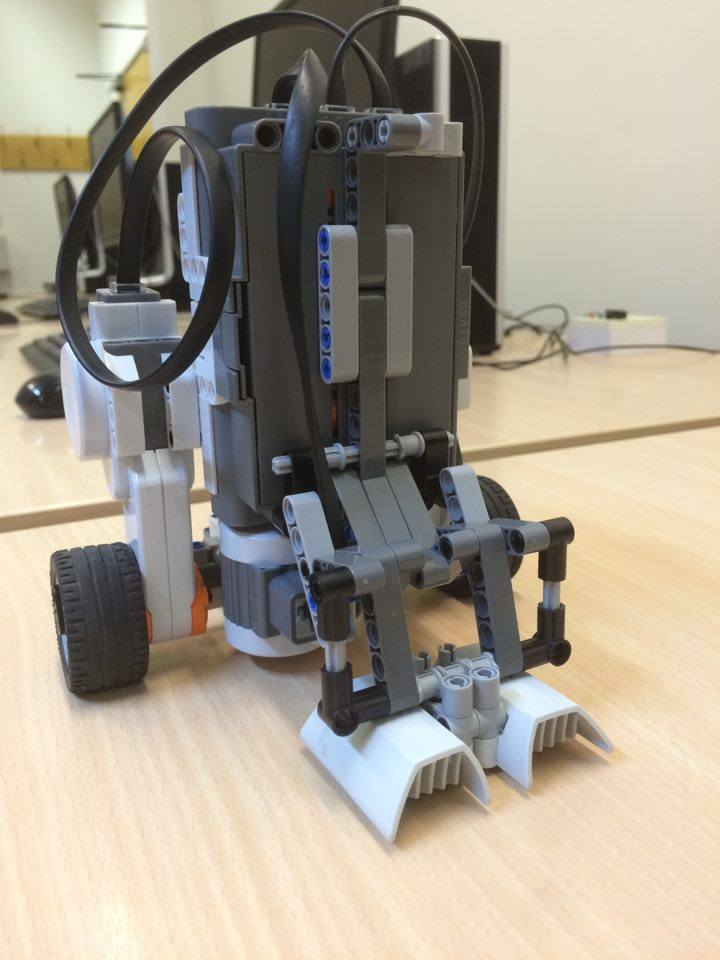
\includegraphics[scale=0.15]{b}
  \caption{Back appearance} \label{fig:backrobot}
  \end{subfigure}
  \caption{Robot configuration.}
  \label{fig:robotconfig}
\end{figure}

\FloatBarrier
